% ------------------------------------------------------------------------------
% TYPO3 CMS 7.0 - What's New - Chapter "Backend User Interface" (English Version)
%
% @author	Michael Schams <schams.net>
% @license	Creative Commons BY-NC-SA 3.0
% @link		http://typo3.org/download/release-notes/whats-new/
% @language	English
% ------------------------------------------------------------------------------
% LTXE-CHAPTER-UID:		8af3f003-d09a4350-9ee0280f-e1de5a69
% LTXE-CHAPTER-NAME:	Backend User Interface
% ------------------------------------------------------------------------------

\section{Administratorski interfejs}
\begin{frame}[fragile]
	\frametitle{Administratorski interfejs }

	\begin{center}\huge{Poglavlje 1:}\end{center}
	\begin{center}\huge{\color{typo3darkgrey}\textbf{Administratorski interfejs}}\end{center}

\end{frame}

% ------------------------------------------------------------------------------
% LTXE-SLIDE-START
% LTXE-SLIDE-UID:		c7e15d2b-d026fd06-55d7edbd-1e63e20d
% LTXE-SLIDE-ORIGIN:	fcbdd27c-e9005dff-0f4dd846-000ea412 English
% LTXE-SLIDE-TITLE:		In General
% LTXE-SLIDE-REFERENCE:	https://forge.typo3.org/issues/62333
% LTXE-SLIDE-REFERENCE:	https://forge.typo3.org/issues/62995
% LTXE-SLIDE-REFERENCE:	https://forge.typo3.org/issues/62158
% LTXE-SLIDE-REFERENCE:	https://forge.typo3.org/issues/61454
% ------------------------------------------------------------------------------

\begin{frame}[fragile]
	\frametitle{Administratorski interfejs}
	\framesubtitle{Uopsteno}

	\begin{itemize}
		\item Znacajne vizuelne promene administratorskog interfejsa
		\item Zasnovan na Twitter Bootstrap-u verzija 3.2.x
		\item Sve ikonice su ponovo uradjene i sada su u stilu "plocica" ("tile")
		\item Ikonice koriste Font Awesome verzija 4.2.x
		\item Navigacija na levoj straini prilagodjena je u skladu sa svojom namenom
		\item Ikonice u navigaciji koriste jasan dizajn, sarolike pozadine sa jednobojnim jasno vidljivim piktogramima u prvom planu, zaobljenih uglova
		\item Sirina navigacije se moze smanjiti tako da samo ikonice budu vidljive

	\end{itemize}

\end{frame}

% ------------------------------------------------------------------------------
% LTXE-SLIDE-START
% LTXE-SLIDE-UID:		6b7b0dd2-917601e0-a4061dcb-4b8ba508
% LTXE-SLIDE-ORIGIN:	0ae980b6-0d2ae6c6-52182f58-aaef69e3 English
% LTXE-SLIDE-TITLE:		Look & Feel (1)
% ------------------------------------------------------------------------------

\begin{frame}[fragile]
	\frametitle{Administratorski interfejs }
	\framesubtitle{Pogledaj i oseti}

	\begin{figure}
		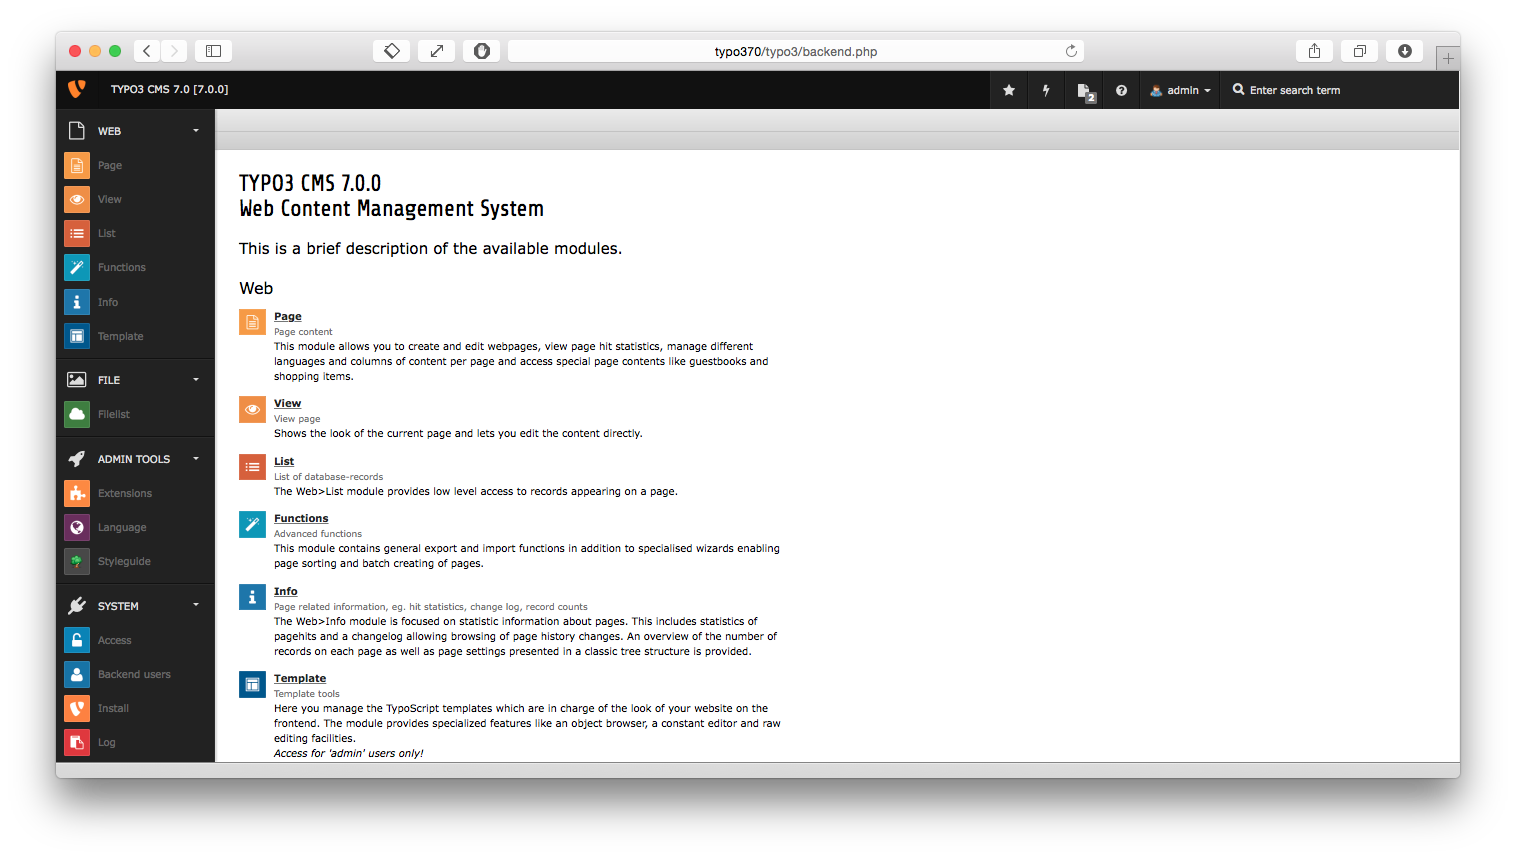
\includegraphics[width=0.90\linewidth]{BackendUserInterface/be-totalscreenshot1.png}
	\end{figure}

\end{frame}

% ------------------------------------------------------------------------------
% LTXE-SLIDE-START
% LTXE-SLIDE-UID:		8dda3de9-68a67ff3-4db6cb71-77f9d009
% LTXE-SLIDE-ORIGIN:	250b123b-2c0bfce4-506f16b0-629baa10 English
% LTXE-SLIDE-TITLE:		Look & Feel (2)
% ------------------------------------------------------------------------------

\begin{frame}[fragile]
	\frametitle{Administratorski interfejs }
	\framesubtitle{Pogledaj i oseti}

	\begin{figure}
		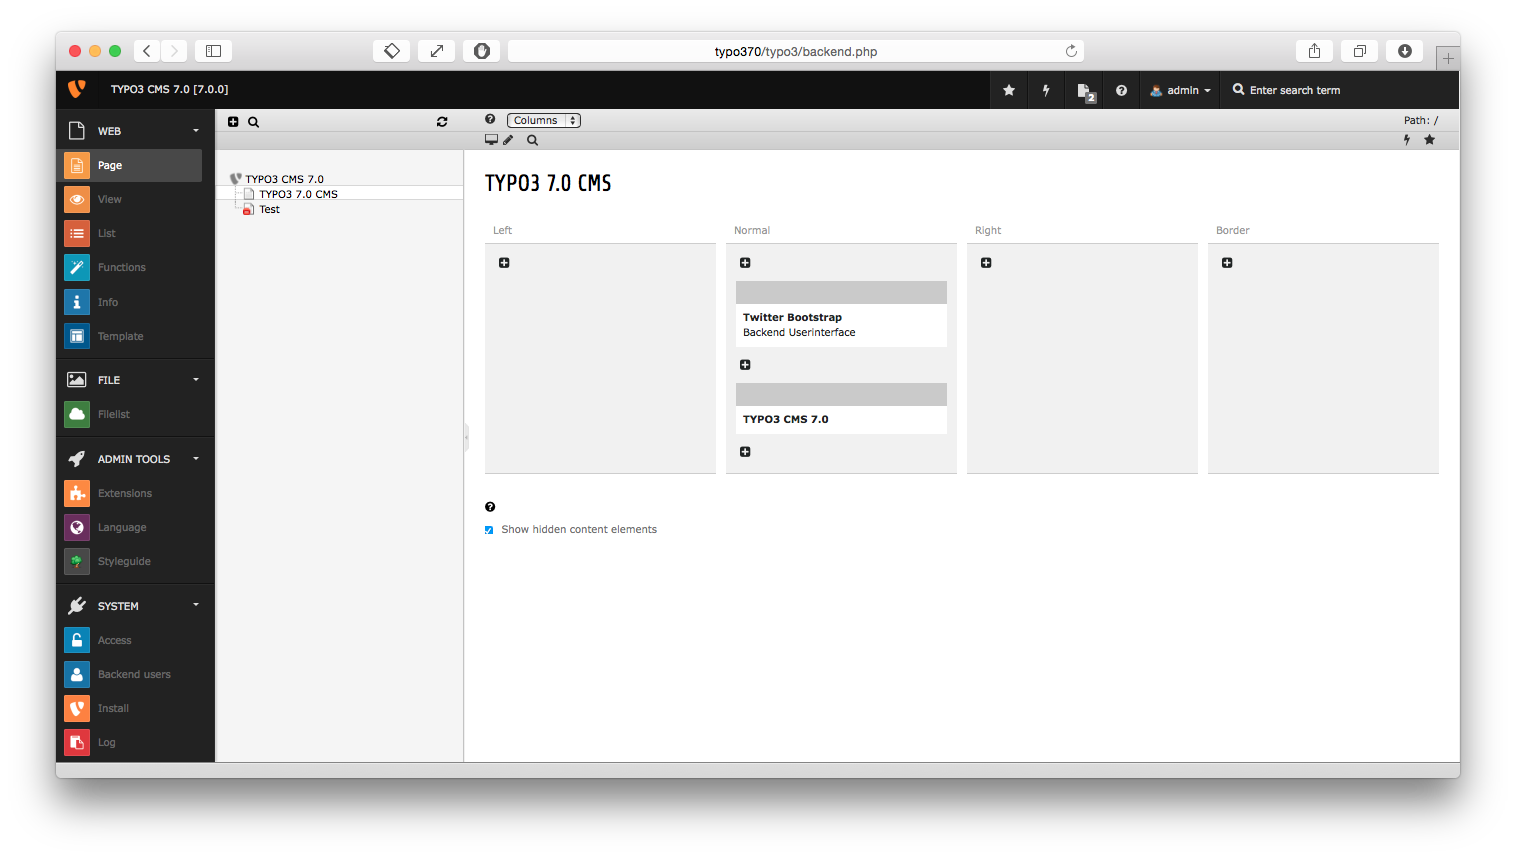
\includegraphics[width=0.90\linewidth]{BackendUserInterface/be-totalscreenshot2.png}
	\end{figure}

\end{frame}

% ------------------------------------------------------------------------------
% LTXE-SLIDE-START
% LTXE-SLIDE-UID:		0cab44d6-ac172cab-665d319c-26dbeadc
% LTXE-SLIDE-ORIGIN:	2d4d33ee-071ae6ed-9f4d0c04-49361364 English
% LTXE-SLIDE-TITLE:		Look & Feel (3)
% ------------------------------------------------------------------------------

\begin{frame}[fragile]
	\frametitle{Administratorski interfejs }
	\framesubtitle{Pogledaj i oseti}

	\begin{figure}
		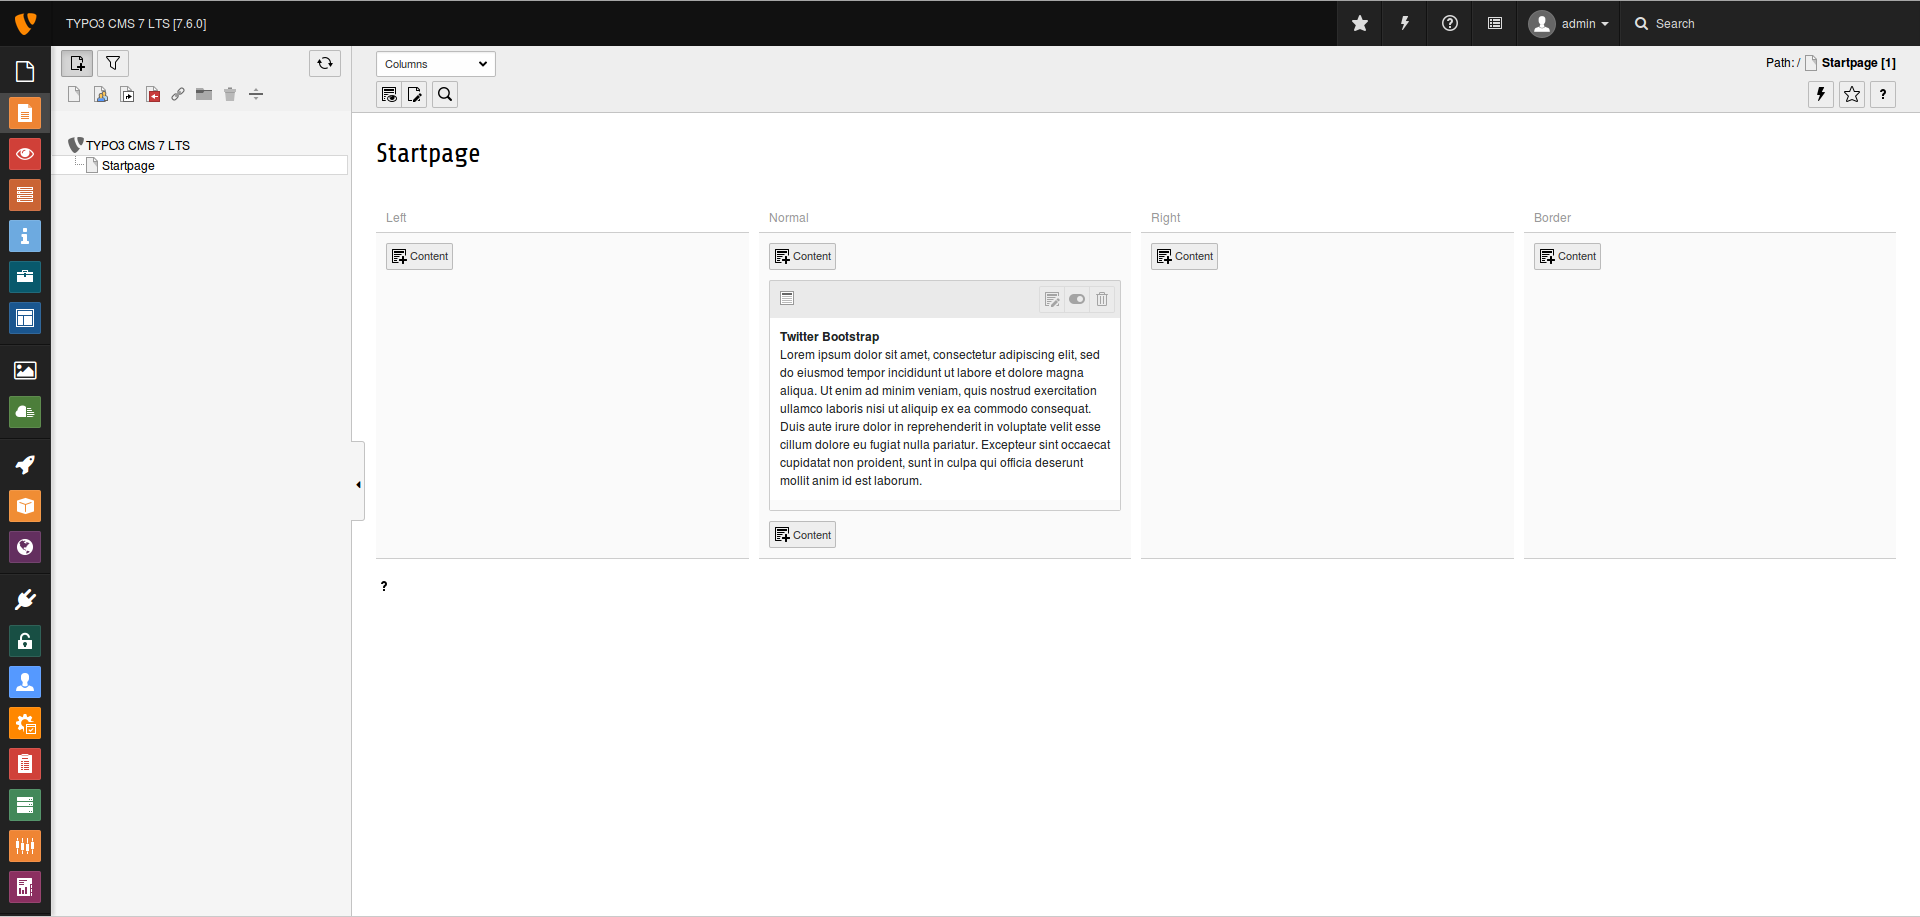
\includegraphics[width=0.90\linewidth]{BackendUserInterface/be-totalscreenshot3.png}
	\end{figure}

\end{frame}

% ------------------------------------------------------------------------------
% LTXE-SLIDE-START
% LTXE-SLIDE-UID:		b4b511eb-eba366d4-e0bdb7ae-e9d58477
% LTXE-SLIDE-ORIGIN:	de58d070-98483f3d-0949f2d1-856a9e7e English
% LTXE-SLIDE-TITLE:		Backend User Login
% ------------------------------------------------------------------------------

\begin{frame}[fragile]
	\frametitle{Administratorski interfejs}
	\framesubtitle{Prijava administratora na administratorski interfejs}

	\begin{figure}
		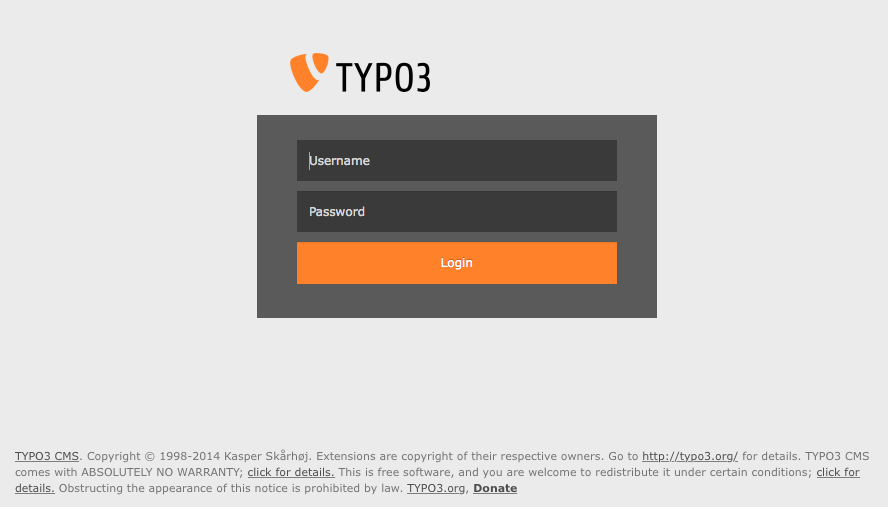
\includegraphics[width=0.80\linewidth]{BackendUserInterface/be-login.png}
	\end{figure}

\end{frame}

% ------------------------------------------------------------------------------
% LTXE-SLIDE-START
% LTXE-SLIDE-UID:		032d3516-ccede3ad-f7fcee90-93023313
% LTXE-SLIDE-ORIGIN:	9baa13c8-78b2f416-28da8e3d-b234e7dc English
% LTXE-SLIDE-TITLE:		Refactor & recolor Modul Menu (Bootstrap)
% LTXE-SLIDE-REFERENCE:	https://forge.typo3.org/issues/62353
% ------------------------------------------------------------------------------

\begin{frame}[fragile]
	\frametitle{Administratorski interfejs}
	\framesubtitle{Gornja navigacija (navigacija modula)}

	\begin{figure}
		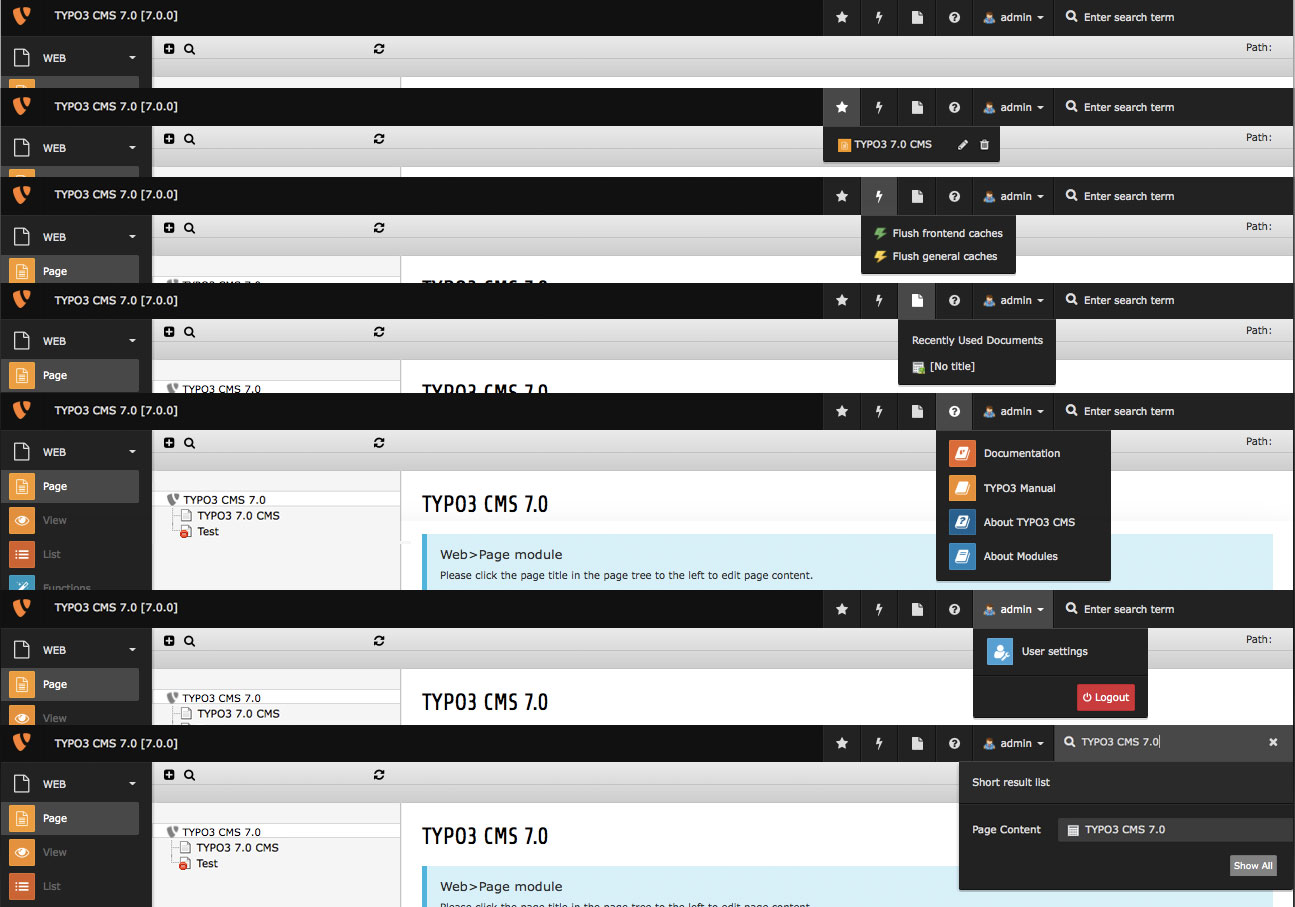
\includegraphics[width=0.70\linewidth]{BackendUserInterface/be-topbar.jpg}
	\end{figure}

\end{frame}

% ------------------------------------------------------------------------------
% LTXE-SLIDE-START
% LTXE-SLIDE-UID:		8eddd971-e3cfedff-6c5e17b9-d0a10bc2
% LTXE-SLIDE-ORIGIN:	4369ae5e-948d1afa-8212cd72-c91c660b English
% LTXE-SLIDE-TITLE:		New List Module Styling
% LTXE-SLIDE-REFERENCE:	https://forge.typo3.org/issues/62963
% ------------------------------------------------------------------------------

\begin{frame}[fragile]
	\frametitle{Administratorski interfejs}
	\framesubtitle{List Modul i Clipboard}

	\begin{figure}
		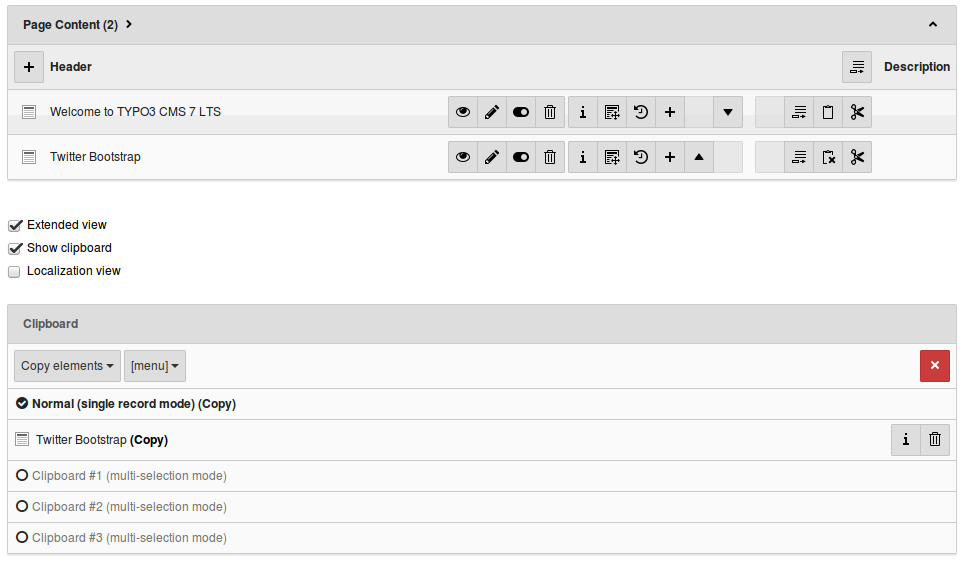
\includegraphics[width=0.80\linewidth]{BackendUserInterface/be-list.png}
	\end{figure}

\end{frame}

% ------------------------------------------------------------------------------
% LTXE-SLIDE-START
% LTXE-SLIDE-UID:		5744a737-507a315c-36c6692b-b0b5d7d1
% LTXE-SLIDE-ORIGIN:	252361f7-e5c42ec2-a90ecd64-4331f02b English
% LTXE-SLIDE-TITLE:		Table Style
% LTXE-SLIDE-REFERENCE:	https://forge.typo3.org/issues/62159
% ------------------------------------------------------------------------------

\begin{frame}[fragile]
	\frametitle{Administratorski interfejs}
	\framesubtitle{Izgled tabela}

	\begin{figure}
		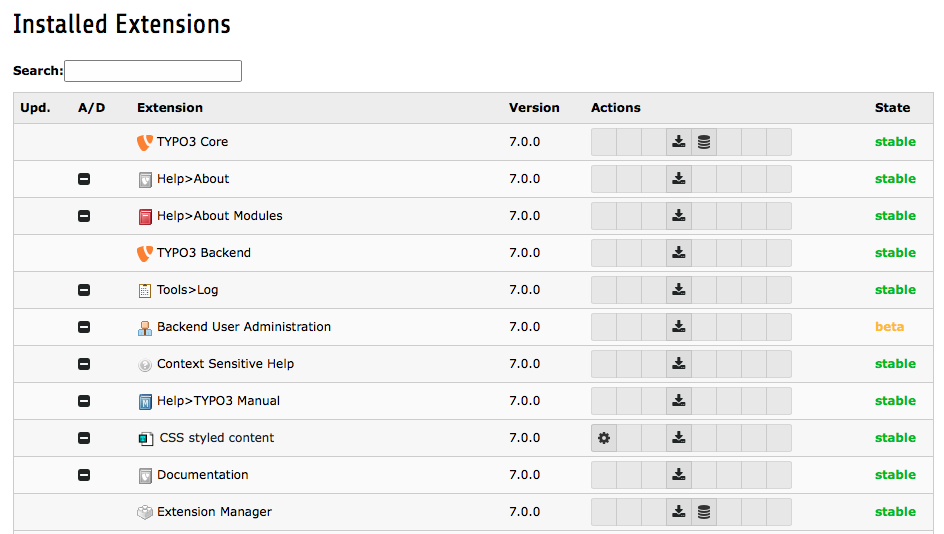
\includegraphics[width=0.99\linewidth]{BackendUserInterface/be-table.png}
	\end{figure}

\end{frame}

% ------------------------------------------------------------------------------
% LTXE-SLIDE-START
% LTXE-SLIDE-UID:		8a182a57-dc8a3d7d-a9cf364e-bc9e6a9c
% LTXE-SLIDE-ORIGIN:	785f717d-a7c4d1dd-f186ca6a-060c1dc4 English
% LTXE-SLIDE-TITLE:		Page And List Search
% LTXE-SLIDE-REFERENCE:	https://forge.typo3.org/issues/59763
% ------------------------------------------------------------------------------

\begin{frame}[fragile]
	\frametitle{Administratorski interfejs}
	\framesubtitle{Pretraga na "List" i "Page" pregledu}

	\begin{itemize}
		\item Klikom na ikonicu lupice otvara se polje za pretragu na "List" i "Page" pregledu \newline
			(funkcija pretrage se ranije nalazila na kraju strane)
	\end{itemize}

	\begin{figure}
		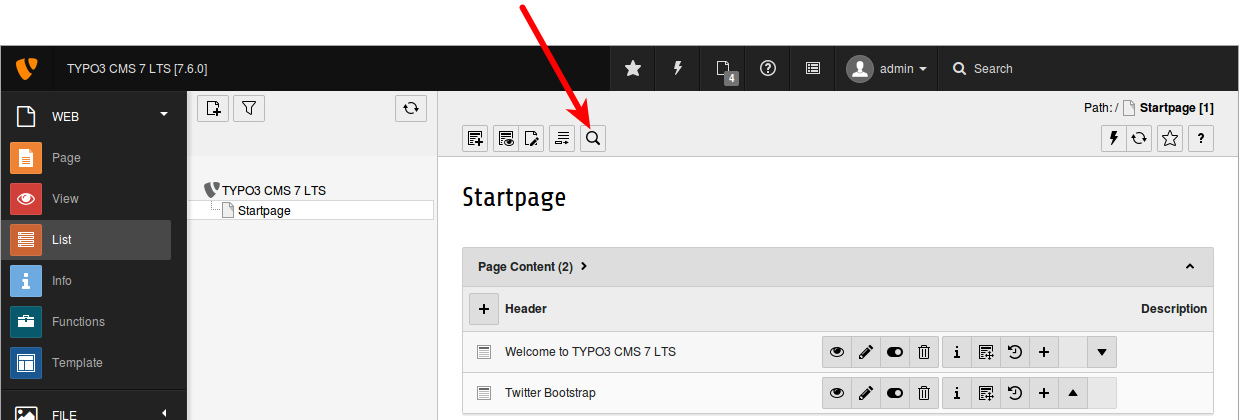
\includegraphics[width=0.95\linewidth]{BackendUserInterface/be-search.jpg}
	\end{figure}

\end{frame}

% ------------------------------------------------------------------------------
% LTXE-SLIDE-START
% LTXE-SLIDE-UID:		208e3ff6-64bb0240-5134c179-391edd56
% LTXE-SLIDE-ORIGIN:	df97fbbf-9ea6c6a9-d9b4c5d4-f8fe1601 English
% LTXE-SLIDE-TITLE:		Migrate Counter of Open Documents to Bootstrap "Badge"
% LTXE-SLIDE-REFERENCE:	https://forge.typo3.org/issues/61675
% ------------------------------------------------------------------------------

\begin{frame}[fragile]
	\frametitle{Administratorski interfejs}
	\framesubtitle{Znacka (Badge) prikazuje sve otvorene dokumente}

	\begin{itemize}
		\item Broj otvorenih dokumenata prikazuje se preko Bootstrap "Znacke"\newline
			(zahteva sistemsko prosirenje "Open Documents")
	\end{itemize}
	\begin{figure}
		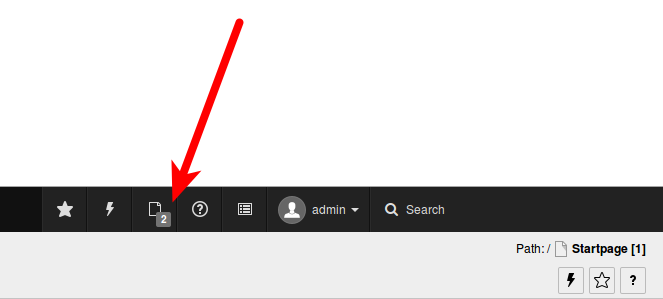
\includegraphics[width=0.75\linewidth]{BackendUserInterface/be-badge.png}
	\end{figure}

\end{frame}

% ------------------------------------------------------------------------------
% LTXE-SLIDE-START
% LTXE-SLIDE-UID:		aedc2a3b-768afb7a-20a0074c-b06457b2
% LTXE-SLIDE-ORIGIN:	a25faae4-8c12c45e-b337b64a-0cf2f53f English
% LTXE-SLIDE-TITLE:		Rebrush FlashMessage
% LTXE-SLIDE-REFERENCE:	https://forge.typo3.org/issues/62580
% ------------------------------------------------------------------------------

\begin{frame}[fragile]
	\frametitle{Administratorski interfejs}
	\framesubtitle{Flash Messages}

	\begin{itemize}
		\item Vizuelni izgled obavestenja je promenjen 
		\item Pojacan je kontrast izmedju teksta i pozadinskog kontejnera
	\end{itemize}

	\begin{columns}[T]
		\begin{column}{.25\textwidth}
			\smaller\hfill 
				\begingroup\color{typo3red}TYPO3 CMS < 7.0\endgroup
			\normalsize
		\end{column}

		\begin{column}{.5\textwidth}
			\begin{figure}\vspace*{-0.6cm}
				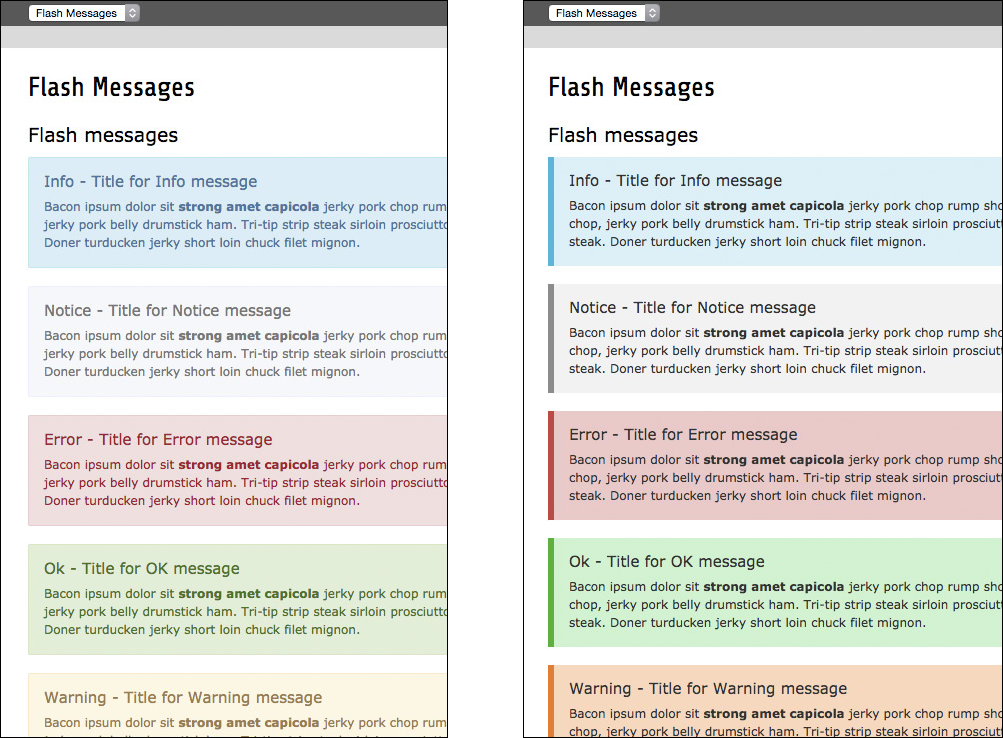
\includegraphics[width=0.99\linewidth]{BackendUserInterface/be-flashmessages.png}
			\end{figure}
		\end{column}

		\begin{column}{.25\textwidth}
			\smaller
				\begingroup\color{typo3red}TYPO3 CMS >= 7.0\endgroup
			\normalsize
		\end{column}

	\end{columns}

\end{frame}

% ------------------------------------------------------------------------------
% LTXE-SLIDE-START
% LTXE-SLIDE-UID:		28793497-35b05f45-aa142f78-8eaeab0b
% LTXE-SLIDE-ORIGIN:	d6a85376-8109aa8c-45a40582-7edb975a English
% LTXE-SLIDE-TITLE:		Video Player in Info Window
% LTXE-SLIDE-REFERENCE:	https://forge.typo3.org/issues/61668
% ------------------------------------------------------------------------------

\begin{frame}[fragile]
	\frametitle{Administratorski interfejs}
	\framesubtitle{Video plejer u info prozoru}
	\begin{itemize}
		\item HTML5 audio i video fajlovi mogu se pustati u info prozoru \newline
			(gde su prikazani meta podaci)
		\begin{figure}
			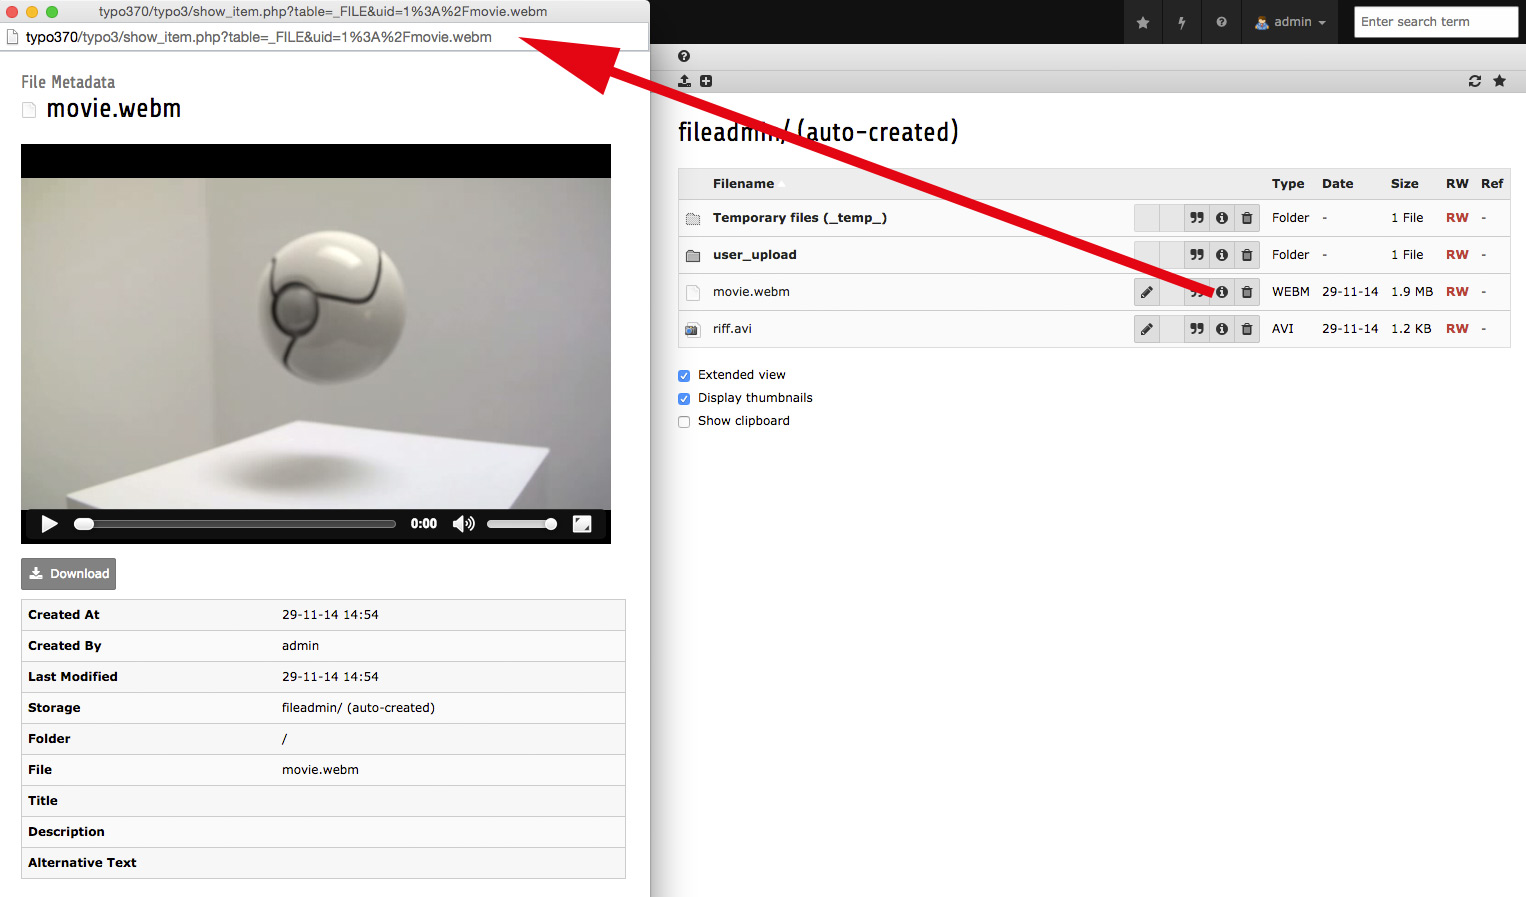
\includegraphics[width=0.70\linewidth]{BackendUserInterface/be-info.jpg}
		\end{figure}

	\end{itemize}

\end{frame}

% ------------------------------------------------------------------------------
